\documentclass{article}

% Packages
\usepackage[utf8]{inputenc}
\usepackage[T1]{fontenc}
\usepackage{times} % Times New Roman font
\usepackage[margin=3cm,left=3.5cm]{geometry} % Set margins
\usepackage{setspace} % For line spacing
\usepackage{graphicx} % For including figures
\usepackage[labelfont=bf]{caption} % Bold figure labels
%\usepackage{natbib} % For bibliography management
\usepackage{hyperref} % For hyperlinks
\usepackage{titling} % For custom title page
\usepackage{float} % For figure placement control
\usepackage[font=small,labelfont=bf]{caption}
\usepackage{tikz}
\usepackage[mode=buildnew]{standalone} 
\usepackage[style=apa, backend=biber]{biblatex}


\addbibresource{references.bib}

\usetikzlibrary{positioning, arrows.meta}

% set spelling to UK English
\usepackage[british]{babel}

% Line spacing (1.5)
\setstretch{1.5}

% Customize hyperref colors
\hypersetup{
    colorlinks=true,
    linkcolor=black,
    citecolor=black,
    urlcolor=blue
}

%\setlength{\parindent}{0pt}

\begin{document}

\begin{titlepage}
    \centering
    \vspace*{3cm}
    
    {\Huge\bfseries A Conservation-Driven Computational Screen for RNA Motifs\par}
    \vspace{2cm}
    
    {\Large Daniel Dachs\par}
    \vspace{1.5cm}
    
    {\large BIOC490\par}
    \vspace{1cm}
    
    {\large Supervisor: Paul Gardner\par}
    \vspace{1cm}
    
    {\large Department of Biochemistry\par}
    {\large University of Otago\par}
    \vspace{1cm}
    
    \vfill
\end{titlepage}

% Main content starts here
\section{Introduction}

RNAs play a wide range of roles in cellular processes, many of which have been harnessed for biotechnological applications, and are likely to have many more functions yet to be discovered.
This project aims to identify novel conserved RNA structural motifs associated with light-sensing gene families in bacteria.
This introduction provides background and rationale for the screening of novel functional RNA motifs in bacterial genomes, and outlines the aims and significance of the project.

\subsection{Ribonucleic Acids}

The central dogma of molecular biology, first articulated by Francis Crick, describes the flow of genetic information: DNA $\rightarrow$ RNA $\rightarrow$ Protein \parencite{Crick1970}.
In this classical view, RNA serves primarily as an intermediate messenger, transcribing genetic information from DNA and translating it into proteins at the ribosome.
However, this perspective underrepresents the diversity in the roles of RNA molecules.

In the hypothetical RNA world, RNA molecules are thought to have performed many of the roles now largely carried out by proteins and DNA, including catalysis, regulation, and information storage \parencite{Kruger1982, Guerrier-Takada1983, Gilbert1986, Breaker2012}.
Although these functions have been largely superseded by proteins and DNA, numerous RNA-based regulatory mechanisms persist in modern organisms.

% Continue with more background sections as needed
\subsection{RNA Structure Determines Function}

RNA molecules, much like the polypeptides that make up proteins, fold into complex structures that enable diverse functions \parencite{Wang2021}.
They typically exist as single-stranded molecules, which can fold back on themselves through intramolecular base pairing to form secondary and tertiary structures.

RNA secondary structure arises from Watson-Crick base pairing (A-U and G-C) and wobble pairing between nucleotides within the same strand \parencite{Tinoco1999}. 
Common secondary structures include hairpins, consisting of a base-paired stem capped by an unpaired loop; internal loops and bulges, made up of unpaired nucleotides within a helical stem; junctions where three or more helical stems converge; and pseudoknots, where nucleotides in a loop pair with regions outside that loop \parencite{Staple2005}.

Beyond secondary structure, RNAs fold into three-dimensional structures through long range interactions \parencite{Batey2004}.
These include base triplets, ribose zippers, A-minor motifs, and tetraloop-receptor interactions, which stabilize compact RNA folds.

The relationship between RNA structure and function is exemplified by riboswitches, a class of regulatory RNAs.
The aptamer domain folds into a specific three-dimensional pocket that selectively binds a target ligand through a combination of electrostatic interactions and shape complementarity \parencite{Kavita2023}.
Ligand binding stabilizes one conformational state over another, thereby modulating transcription termination or initiation.
This allosteric mechanism, whereby binding at an aptamer site affects a distal functional region, demonstrates how RNA structure enables regulatory function.

\subsection{Functional RNAs in Biology and Biotechnology}

The diverse functional roles of RNA are driven by their structural and reactive diversity. 
Naturally occurring functional RNAs include purely RNA systems, riboswitches and ribozymes, and those in complexes with proteins, while \emph{in vitro} selected RNAs include fluorogens and aptazymes \parencite{Micura2020}.

\subsubsection*{Ribonucleoprotein Complexes}

While some RNAs function independently, many operate in ribonucleoprotein (RNP) complexes.
The ribosome is one such RNP with critical function in all cells.
This large complex catalyses peptide bond formation, with ribosomal RNA (rRNA) forming the catalytic core, while ribosomal proteins provide structural support and regulatory functionality \parencite{Wahl2009}.
Spliceosomes are another example of essential RNPs in eukaryotes \parencite{Wahl2009}.

In bacteria, several classes of RNPs mediate post-transcriptional regulation. 
Small regulatory RNAs (sRNAs) often require the RNA chaperone Hfq to facilitate base pairing with target mRNAs, thereby modulating transcript stability \parencite{Vogel2006}.

CRISPR-Cas systems exemplify the complexity of bacterial RNPs.
CRISPR RNAs (crRNAs) guide Cas nucleases to complementary DNA or RNA targets, enabling sequence-specific nucleic acid cleavage \parencite{Barrangou2007}.
This mechanism has famously been repurposed as a gene-editing tool \parencite{Jinek2012}.

\subsubsection*{Ribozymes}

Ribozymes are catalytic RNAs that accelerate chemical reactions, much like protein enzymes.
Beyond the ribosome and spliceosome, several small self-cleaving ribozymes exist in nature, including the hammerhead, hairpin, hepatitis delta virus (HDV), glmS, twister, and pistol ribozymes \parencite{Roth2014, Weinberg2015, Micura2020}. 

\subsubsection*{Riboswitches}

%Including light sensitive/related, give some importance of these

Riboswitches are structured RNA domains that regulate gene expression in response to some stimuli, often the presence of a metabolite \parencite{Breaker2023}.
Although seemingly less abundant than protein factors that perform similar functions, riboswitches are recognized as important regulatory elements across all domains of life.
They are typically embedded within messenger RNAs and control gene expression through ligand-induced conformational changes.

Riboswitch mechanisms vary widely.
Figure~\ref{fig:riboswitch-mechanism} illustrates several experimentally validated regulatory strategies \parencite{Kavita2023}.

\begin{figure}[H]
    \centering
    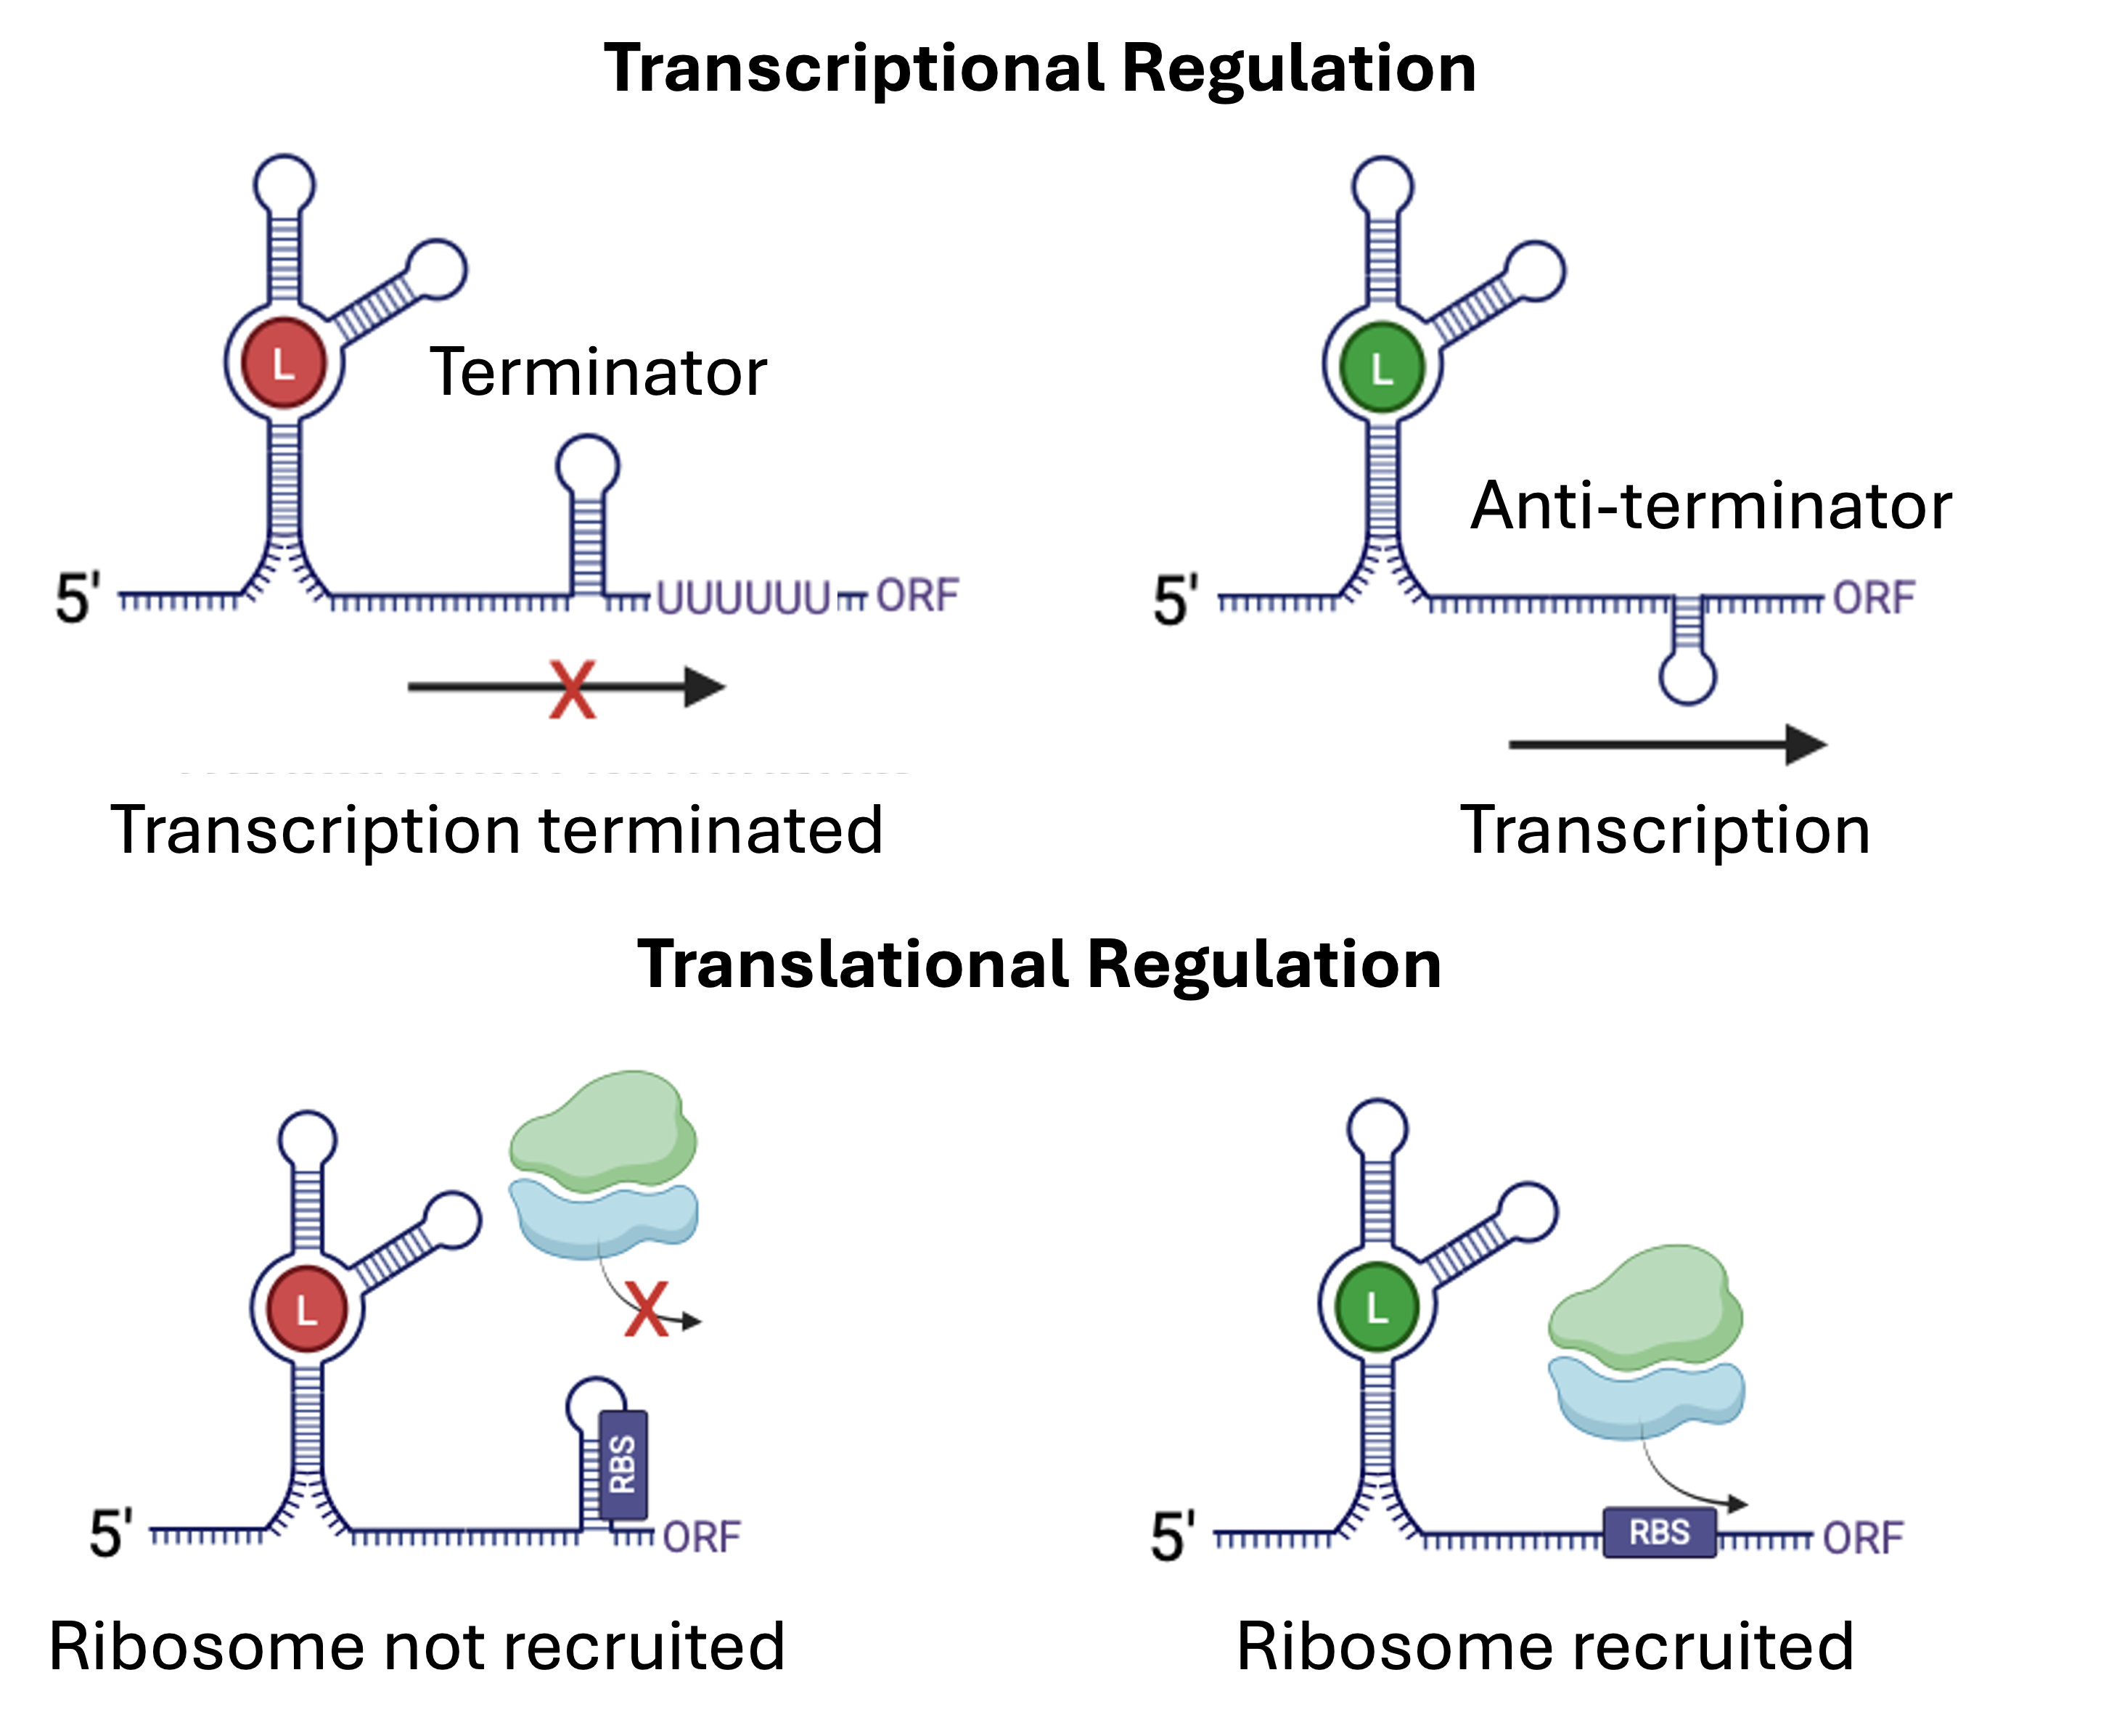
\includegraphics[width=0.8\textwidth]{figures/riboswitch-mechanism.png}
    \caption{\textbf{Typical riboswitch regulatory mechanisms.} 
    Riboswitches control gene expression through ligand-induced conformational changes that affect either transcription or translation.
    Ligands ("L") bind aptamers resulting in 
    \textbf{Transcriptional control (top):} Riboswitches can either promote an early termination when ligand-bound (left) or prevent termination (right) allowing transcription through the ORF. 
    \textbf{Translational control (bottom):} Riboswitches can either make the ribosome binding site less accessible (left) or more accessible (right) when ligand-bound.
    ORF = open reading frame; RBS = ribosome binding site. 
    Created in  https://BioRender.com}
    \label{fig:riboswitch-mechanism}
\end{figure}

Transcriptional riboswitches control formation of Rho-independent terminators—intrinsic termination structures consisting of a hairpin followed by a uridine-rich tract. 
Depending on the riboswitch, ligand binding may promote terminator formation or stabilize an antiterminator structure, enabling transcriptional read-through.
Similarly, translational riboswitches can sequester or expose the ribosome-binding site in response to ligand binding \parencite{Breaker2023}.

\subsubsection*{Biotechnological Applications}

RNA has been central to several majoy biotechnological breakthroughs. 
CRISPR-Cas9 gene editing harnesses guide RNAs for programmable genome modification \parencite{Jinek2012}. 
mRNA vaccines against COVID-19 demonstrated the therapeutic potential of synthetic mRNAs \parencite{Polack2020}. 
RNA interference (RNAi) enables targeted gene silencing in research and therapeutics \parencite{Fire1998}.

RNA aptamers such as Spinach bind fluorogenic compounds and fluoresce upon binding, enabling RNA visualization in living cells \parencite{Paige2011}.
The photoriboswitch Werewolf-1, generated through \emph{in vitro} selection, responds to light by binding photoisomerizable ligands, offering potential for optogenetic control of gene expression \parencite{Rotstan2020}.
These RNAs, involved in fluorescence and photoreception, have broad relevance for medical research, biotechnology, and agricultural applications \parencite{Micura2020}.

\subsection{Current Approaches to Functional RNA Discovery}

It is predicted that a large number of riboswitches remain undiscovered, potentially on the order of thousands \parencite{Kavita2023}.
Ronald Breaker and colleagues have pioneered systematic riboswitch and ribozyme discovery, identifying over 55 distinct riboswitch classes to date \parencite{Breaker2022}.
Other major RNA-related discoveries, such as ribosomes and CRISPR-Cas systems, occurred through more exploratory research approaches \parencite{Brück2025}.

\subsubsection*{Experimental Approaches}

Transcriptome mapping approaches have proven successful for unbiased riboswitch discovery. 
Term-seq maps RNA 3' termini genome-wide to identify premature transcription termination sites characteristic of riboswitches and attenuators \parencite{Dar2016}. This approach discovered numerous antibiotic-responsive riboswitches controlling resistance genes in bacterial pathogens and the human microbiome. 
This approach has uncovered numerous antibiotic-responsive riboswitches controlling resistance genes in bacterial pathogens and within the human microbiome.
RNA structure probing methods characterize secondary structures, tertiary interactions, and dynamic conformational changes. 
SHAPE-seq (Selective 2'-Hydroxyl Acylation analysed by Primer Extension Sequencing) chemically modifies unpaired nucleotides, enabling genome-wide structure mapping \parencite{Lucks2011}. 
This approach can identify structured regions throughout transcriptomes, revealing RNA switches, ribozymes, and protein-binding sites.
DMS-MaPseq extends this approach to structural probing \emph{in vivo} \parencite{Zubradt2017}.
A variety of methods exist for studying protein-RNA interactions from both protein- and RNA-centric approaches \parencite{Yi2025}.

While powerful for validation and mechanistic characterization, experimental approaches are labour-intensive, may miss RNAs with unknown functions, and are difficult to scale across many organisms.

\subsubsection*{\emph{In Vitro} Selection and Computational Design}

\emph{In vitro} selection (SELEX) generates novel functional RNAs by applying selective pressure to a library of random sequences.
This technique was used in the generation of the photoriboswitch, Werewolf-1 \parencite{Rotstan2020}.
Generation of synthetic functional RNAs by computational design has also been reported, with tools like RfamGen and RhoDesign \parencite{Sumi2024}.

Many RNA discoveries, including CRISPR-Cas systems, mRNA vaccine strategies and many catalytic RNAs were however discovered in nature, not designed \emph{de novo} \parencite{Micura2020,Barrangou2007}.
Beyond biotechnology, fundamental understanding of natural RNA-based systems has value, for example the discovery of flouride sensing riboswitches in bacteria \parencite{}

\subsubsection*{Computational Approaches}

Bioinformatic sequence-based searches using tools like BLAST identify homologous sequences, but many functional RNAs have divergent sequences detectable only through structural conservation.
Structure based searches have proven successful, like the bioinformatic search for twister ribozymes by \textcite{Roth2014} discovering roughly 2,700 ribozymes.
These techniques search on sequence and secondary structure patterns, but require existing alignments and structure models, limiting their utility for discovering entirely novel RNA classes.

RNA structure prediction remains a challenging problem, particularly when given a single sequence and no homology structures are known, as would be the case with a genome wide search for novel RNA structures in a single species.
Comparative approaches using multiple homologous sequences provide greater predictive power for RNA structure inference \parencite{Kagaya2026}.

Comparative genomics leverages evolutionary conservation of RNA structures across related species, enabling the identification of conserved structural features.
These conserved features are termed RNA motifs, regions showing evidence of selective constraint on structure, indicating potential functional importance. 
Such motifs may represent riboswitches, ribozymes, or other classes of functional RNAs.

Zasha Weinberg's lab has had notable successes with their tool CMfinder, \textcite{Yao2006}, which identifies conserved RNA secondary structures using a comparative genomics approach.
The \textcite{Sack2025} paper, also from the Weinberg lab, recently identified 16 new structured RNA classes in plants using a CMfinder-based bioinformatic screen.
This study focused on structured RNAs involved in alternative splicing.

\textcite{Roth2014} also employed CMfinder to identify a new class of self cleaving ribozymes, the twister ribozyme, which has since been found to be widespread in nature.
In that paper hammerhead and twister ribozymes were observed to commonly reside near each other and to certain protein coding genes, although noting it still a biological mystery. 
\textcite{Weinberg2015} followed up on this observation with a screening of sequences nearby known ribozyme and ribozyme associated protein domain coding regions.
This approach successfully identified additional ribozyme classes including pistol and hatchet.

\subsection{Gene Family-Targeted Searches}

Beyond the successes of gene family-targeted searches with CMfinder, there is precedent for riboswitches being encoded upstream of certain gene families \parencite{Micura2020, Kavita2023}.
This approach also provides a less computationally intensive alternative to genome-wide screens, allowing for wider searches across more species.
Harnessing the power of evolutionary conservation and leveraging the biological assumption that functionally related genes (i.e. with domain homology) may share regulatory mechanisms.

Due to its potential importance in biotechnology this project will be screening for conserved RNA structures located near light-sensing gene families.
Light-sensing systems in bacteria often involve complex regulatory networks, and RNA-based mechanisms have been shown to play roles in light acclimation responses in cyanobacteria \parencite{Hihara2015}.

A recent study by a group in Copenhagen, \textcite{Geissler2026}, describes a bioinformatic screen similar to the one undertaken here.
In that work orthologous cyanobacteria genes involved in photosynthetic pathways were targeted for nearby conserved RNA structure discovery using CMfinder.
Approximately 400 novel conserved RNA structures were identified.

\subsection{Bacterial Genomes as a Search Space}

Riboswitches have been most extensively discovered and experimentally validated in bacteria and seem to rarely have homologs in eukaryotes \parencite{Kavita2023}.
This makes bacteria a reasonable domain for riboswitch discovery efforts.

Extensive phylogenetic diversity is available among sequenced bacterial genomes.
As of April 2026, over 870,000 bacterial genomes spanning 180,000 bacterial species clusters have been sequenced and organised in databases such as the Genome Taxonomy Database \parencite{GTDB2026}.
This represents vast evolutionary distances, bacteria diverged over 3 billion years ago, providing the deep phylogenies necessary for detecting conserved structures through covariation analysis.

Bacterial regulatory mechanisms are generally simpler than eukaryotic systems, with less complex post-transcriptional processing and more direct coupling between transcription and translation. 
This simplifies both computational predictions and experimental validation.

% Project aims (should be about half a page)
\subsection{Aims}

The overarching aim is to discover novel functional RNA motifs associated with bacterial light-sensing systems by leveraging comparative genomics. 
Gene-family-targeted approaches offer a computationally tractable approach for identifying regulatory elements linked to specific biological pathways. 
Light-sensing gene families are of particular interest due to their importance in environmental adaptation and their potential relevance to biotechnological applications. 
Identifying conserved RNA structures associated with these genes may reveal previously uncharacterized regulatory mechanisms.

The first aim of this project is therefore to identify evolutionarily conserved RNA structural motifs located near light-sensing gene families across diverse bacterial lineages. 
By examining intergenic and transcript regions associated with these genes, the project aims to predict conserved RNA secondary structures using comparative genomics approaches that identify covariation patterns indicative of selective constraint.
These may represent riboswitches, ribozymes, or other regulatory elements. 

The second aim is to develop a generalizable comparative genomics pipeline using modern tools, capable of systematically screening for conserved RNA structures linked to specific protein domain families. 
This pipeline is intended to be reusable and adaptable for future studies, targeting additional gene families or biological pathways. 

Together, these aims will contribute both new candidate RNA motifs and a methodological platform for search for structured RNAs in nature.

\subsection{Hypothesis}

Evolutionarily conserved structural motifs within transcripts associated with specific gene families represent functional regulatory elements maintained by natural selection.
These elements may employ diverse mechanisms, including ligand-dependent structural switching (riboswitches), catalytic self-cleavage (ribozymes), protein binding, or other structure-based regulatory strategies, to control gene expression.

% Bibliography
\newpage
\printbibliography

\end{document}
